%%=============================================================================
%% Inleiding
%%=============================================================================

\chapter{Inleiding}
\label{ch:inleiding}

In deze sectie wordt de context en achtergrond rond deze bachelorproef meegedeeld. Alsook wordt de probleemstelling, de onderzoeksvragen en onderzoeksdoelstellingen uitgelegd. Daarbovenop wordt de opzet van de bachelorproef verduidelijkt. 

\section{Probleemstelling}
\label{sec:probleemstelling}

Alhoewel meer en meer processen wereldwijd volledig digitaal plaatsvinden, worden toch nog een grote deel van procedures en data opslag uitgevoerd op niet-digitale manieren. Zo krijgen de meeste mensen hun factures nog steeds per brief. Volgens de \textcite{FederaleOverheidsdienstEconomie} blijft het verzenden of ontvangen van facturen op papier een zeer gangbare praktijk. Zo verstuurde 90 \% van de bedrijven er en 97 \% ontving er in 2017. Daarbovenop worden kassatickets nog steeds afgedrukt op papier, en notities nemen op papier blijft de populaire keuze hoewel er tal van notitie-apps bestaan. Deze voorbeelden tonen aan dat essentiële data nog massaal op een niet-digitale, en dus niet-automatisch verwerkbare media bewaard wordt, namelijk op papier.

Tot enkele jaren geleden was dit probleem niet zo beduidend maar nu meer digitale
platformen voor dataverwerking gebruikt worden, is het omzetten van data op papier naar
digitale data, m.a.w. het digitalisatieproces steeds belangrijker geworden.

Hierdoor werden tal van digitalisatiesofwareproducten ontwikkeld, zoals Abby FineReader
en Adobe Acrobat Pro DC. Hoewel deze software producten veel features hebben, zoals \Gls{OCR}, tabelherkenning, formulierherkenning, etc, zijn ze betalend en closed source. Wat als gevolg heeft dat ze voor bedrijven een merkbare kost met zich meebrengen, naast een privacy- en veiligheidsrisico aangezien het om closed source software gaat.

% TODO: prijzen van finereader toe, voordelen van open source software

Sommige bedrijven enkele van hun digitalisatie oplossingen open source gemaakt, zoals Google met diens bekende OCR-software, Tesseract OCR, die door iedereen gebruikt kan worden om tekst in foto’s om te zetten in tekstdata. Hoewel \Gls{OCR} op zich zeer belangrijk is voor digitalisatie, is het niet voldoende voor volledige digitalisatie. Zo kan men de relatie tussen verschillende documententiteiten, die normaal gezien grafisch wordt verduidelijkt, enkel met \Gls{OCR} digitaal niet overbrengen. In documenten worden relaties tussen woorden meestal a.d.h.v. een tabel verduidelijkt. Door gebruik te maken van \Gls{OCR}, verkrijgt men wel de tekst binnen een tabel, maar men verliest essentiële informatie rond de woorden, namelijk tot welke rij en kolom ze behoorden. Het valt tenslotte niet onder de verantwoordelijkheid van OCR-engines om naast tekstherkenning, ook nog tabeltransformatie uit te voeren.

\begin{figure}[h]
    \centering
    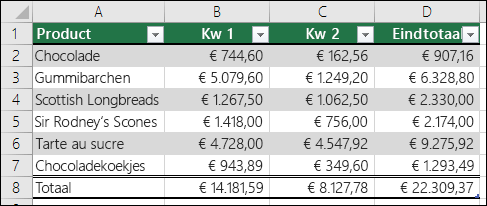
\includegraphics[width=0.8\textwidth]{img/tabel_verduidelijking_relaties_woorden.png}
    \caption{Voorbeeld van een tabelafbeelding. Bron: support.microsoft.com}
    \label{fig:tabel_verduidelijking_relaties_woorden}
\end{figure}

Indien men bij tabelafbeelding \ref{fig:tabel_verduidelijking_relaties_woorden} enkel \Gls{OCR} voor digitalisatie zou gebruiken, dan verkrijgt men wel de tekst, zoals de tekststukken zoals ``Kw 1``, ``Kw 2``, ``€744,60``, ``€ 162,56``, en meer, maar men behoudt niet de relatie tussen de tekststukken. Hierdoor zal men enkel met \Gls{OCR} niet te weten komen of de verkoopbedrag van € 744,60 bij de eerste kwartaal behoort, of bij de tweede, wat essentiële informatie is voor verdere financïele analyse.

Tot heden bestaat er geen open source oplossing die tabellen in foto's transformeert naar digitale tabellen, m.a.w. naar digitale structuren waarbij de tekst, evenals de relatie tussen de verschillende teksten getransformeerd wordt. Daarom werd er voor deze bachelorproef beslist om een proof-of-concept van een tabeltransformatiesoftware te creëren die bij een foto automatisch tabellen detecteert en deze tabellen digitaliseert.

Een belangrijke professionele toepassing van digitale tabeltransformatie is het digitaliseren van ingescande medicatieschema’s, door technologiebdrijven zoals Into.care die zich bezig houden met digitale gezondheidszorg. Medicatieschema's worden in de gezonheidszorg gebruikt om medicatiedata voor patiënten te bewaren en weer te geven. Volgens de definitie van Apothekersnetwerk \autocite{ApothekersNetwerk2013} is het medicatieschema een geheel van gestandaardiseerde informatie over de actieve medicatie van een patient, met inbegrip van de identiteit van de geneesmiddelen, hun dosering, indicatie, relevante gebruiksaanwijzingen en bijkomende informatie waar nodig. Het omvat zowel voorgeschreven als niet-voorgeschreven geneesmiddelen en voedingssupplementen.

Deze oplijsting van de actieve medicatie van de patient is niet enkel een essentieel hulpmiddel voor de patient bij de correct inname van medicatie maar ook voor medische professionelen om bv. over- of onderdosering, dubbelmedicatie, en andere geneesmiddelgebonden problemen te voorkomen. Ook wordt het gebruikt bij de communicatie tussen zorgverstrekkers. Het medicatieschema wordt eveneens door verpleegsters geraadpleegd voor het klaarzetten van de medicatie.

\begin{figure}[h]
    \centering
    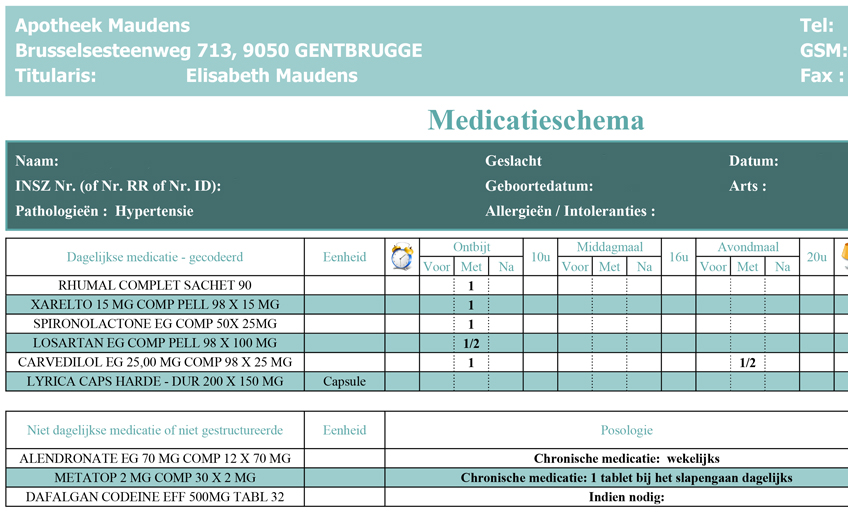
\includegraphics[width=1\textwidth]{img/voorbeeld_medicatieschema.jpg}
    \caption{Voorbeeld medicatieschema. Bron: apotheektsjoen.be}
    \label{fig:voorbeeld_medicatieschema}
\end{figure}

Zoals men in figuur \ref{fig:voorbeeld_medicatieschema} kan zien, wordt dit schema grafisch in tabulaire vorm gepresenteerd. Echter is de lay-out hiervan niet gestandaardiseerd; afhankelijk van de apotheker of andere zorgverstrekker worden andere kolomnamen, kolomverdeling, rand- en verdelingstijl, celgrootte en andere tabelelementen aangewend. Dit bemoeilijkt ernstig het ontwikkelen van een transformatiesysteem die ingescande medicatieschema’s omzet in instanties van een uniform digitale datastructuur in bv. XML- of JSON-formaat voor digitale verwerking van de medicatiedata in gezondheidszorgplatformen.

Een open source tabeltransformatiesoftware zal automatisch medicatieschema’s kunnen omzetten in een uniform digitale datastructuur. Hierdoor zal er geen manuele werk uitgevoerd moeten worden, wat tijd- en kostenreductie als positieve gevolgd heeft. Daarbovenop, omdat het open source zal zijn, zal men verzekerd zijn dat Into.care niet zal te maken hebben met softwarelicentiekosten of privacyschending.

% TODO: schema tabeltransformatiesoftware die medicatieschema omzet in JSON

Hoewel het digitaliseren van medicatieschema’s een belangrijke toepassing is, zijn er tal van andere potentiële toepassingen, aangezien tabellen zo vaak gebruikt worden. Zo zou men tabeltransformatie eveneens kunnen gebruiken voor het inscannen van kassatickets, het analyseren van een sudokuspel, het digitaal weergeven van een - op een whiteboard gemarkeerde - matrix voor online leerplatformen, het verwerken van een foto van een voedingswaardetabel op de verpakking van voedsel, en meer. Het is duidelijk dat een open source tabeltransformatiesoftware een beduidende universeel meerwaarde zal aanbieden.

% TODO: compilatie voorbeelden tabellen

\section{Onderzoeksvraag}
\label{sec:onderzoeksvraag}

Men kan zich bij tabeltransformatie, en dus bij dit onderzoek, enkele vragen stellen.

\begin{itemize}
    \item Uit welke processen bestaat tabeltransformatie? In welke volgorde deze plaats?
    \item Hoe kan men de performantie van tabeltransformatiesoftware best evalueren?
    \item Is preprocessing van de afbeelding nodig om de nauwkeurigheid van de resultaten te bewaren? Indien ja, uit welke stappen bestaat deze preprocessing?
    \item Analoog, is postprocessing van de verkregen tabel noodzakelijk? Indien ja, uit welke stappen bestaat deze postprocessing?
    \item Op welke manieren kan men de resultaten verbeteren, indien men in bezit is van domeinkennis? Zo zou men bijvoorbeeld kennis van de gezondheidszorg kunnnen gebruiken om medicatieschema’s nauwkeuriger te digtaliseren.
\end{itemize}

\section{Onderzoeksdoelstelling}
\label{sec:onderzoeksdoelstelling}

Aangezien het doel van deze studie het creëren van een end-to-end tabeltransformatie-tool is, zal er niet alleen gestreefd worden subprocessen zoals \Gls{OCR} of preprocessing geïsoleerd te bestuderen maar evenwel de subprocessen te implementeren in code. Eveneens is het de bedoeling dat de componenten met elkaar op een geïntegreerde manier zullen kunnen functioneren.

Dit betekent dat de prototype niet enkel zal bestaan uit tabelanalysesoftware, maar alsook uit een \Gls{GUI}, een backend server, een preprocessing pipeline, en meer. 

\section{Opzet van deze bachelorproef}
\label{sec:opzet-bachelorproef}

% Het is gebruikelijk aan het einde van de inleiding een overzicht te
% geven van de opbouw van de rest van de tekst. Deze sectie bevat al een aanzet
% die je kan aanvullen/aanpassen in functie van je eigen tekst.

De rest van deze bachelorproef is als volgt opgebouwd:

In Hoofdstuk~\ref{ch:stand-van-zaken} wordt een overzicht gegeven van de stand van zaken binnen het onderzoeksdomein, op basis van een literatuurstudie.

Verder wordt in Hoofdstuk~\ref{ch:methodologie} de methodologie toegelicht en worden de gebruikte onderzoekstechnieken besproken om een antwoord te kunnen formuleren op de onderzoeksvragen.

In Hoofdstuk~\ref{ch:proof-of-concept} wordt vervolgens de architectuur van de proof of concept uitgelegd. Eveneens worden de verschillende algoritmen in detail besproken.

Verder worden in Hoofdstuk~\ref{ch:resultaten} de met de proof of concept verkregen resultaten besproken en vergeleken.

In Hoofdstuk~\ref{ch:optimalisatiemogelijkheden} worden enkele optimalisatiemogelijkheden om de nauwkeurigheid van het systeem te verhoden, besproken.

En tenslotten in Hoofdstuk~\ref{ch:conclusie},  wordt de conclusie gegeven en een antwoord geformuleerd op de onderzoeksvragen. Daarbij wordt ook een aanzet gegeven voor toekomstig onderzoek binnen dit domein.


